\documentclass[11pt]{article}
\usepackage[UKenglish]{babel}
\usepackage{graphicx}
\usepackage{amsmath}

\usepackage{parskip}
% same as: Dutch style of paragraph formatting, i.e. no indents. 
%\setlength{\parskip}{1.3ex plus 0.2ex minus 0.2ex}
%\setlength{\parindent}{0pt}

\begin{document}



%%%% Title page %%%%

\begin{titlepage}
\begin{center}

\vspace{2.5cm}

\begin{huge}
Optimizing Artificial Force Fields for Autonomous Drones in Figure-eight Task using Reinforcement Learning
\end{huge}

\vspace{1.5cm}
Martijn F.W. van der Veen\\
5964008

\vspace{1cm}
\textbf{Bachelor thesis}\\
Credits: 15 EC

\vspace{0.25cm}
Bacheloropleiding Kunstmatige Intelligentie

\vspace{0.25cm}
University of Amsterdam\\
Faculty of Science\\
Science Park 904\\
1098 XH Amsterdam

\vspace{2cm}
\emph{Supervisor}\\
Dr. A. Visser

\vspace{0.25cm}
Intelligent Systems Lab Amsterdam\\
Faculty of Science\\
University of Amsterdam\\
Room C3.237\\
Science Park 904\\
NL 1098 XH Amsterdam

\vspace{1.5cm}
July 28th, 2010

\end{center}
\end{titlepage}

\pagebreak



%%%% Abstract %%%%
\pagestyle{empty} % no page number
\begin{abstract}
%todo
\end{abstract}
%keywords
\pagebreak

%%%% Acknowledgments %%%%
%\section{Acknowledgments}
% - Arnoud, Nick, Robrecht

%%%% Contents %%%%
\pagestyle{empty} % no page number
\tableofcontents
\pagebreak



%%%% Introduction %%%%
\setcounter{page}{2}
\section{Introduction}
\label{sec:intro}

% - problem sketch
% - research question

People seem to think that the goal of Artificial Intelligence is the creation of autonomous, intelligent robots. According to researchers in the field of robotics, it seems indeed to be the \emph{ultimate} goal. Although a lot of progress has been made in the last couple of decades, the ultimate goal still appears far from reached. Different sub-problems ask for different algorithms, and `the best' framework does not (yet) exists. In the course of time, a lot of algorithms have been invented and are investigated exhaustively, and some became part of the standard toolbox\footnote{As an example, the SLAM algorithm, for both mapping and localizing in unknown environments, is being used frequently}. Since there still are a lot of challenges, existing ideas are being shaped and new algorithms are being proposed, and tested on both existing and new problems.

One challenge within robotics is the simple task of autonomous navigating towards a goal, without hitting obstacles. One of the proposed methods that try to solve this task uses artificial forces to guide the robot. The robot is attracted by the goal, while obstacles spread a repelling force. The approach works, but does not give an optimal path. This leads to the question whether the forces, which look like a good starting point, could be improved by learning.

A well-known approach within robotics for learning is reinforcement learning. This semi-unsupervised learning methodology uses the intuitive notion of reward and punishment received from the environment to learn optimal actions for possible situations (i.e., locations within the environment). The objective of this thesis is to take the forces, or force field, as initial set up, and improve it using reinforcement learning. The improved force field should lead to better paths that cause the robot to move faster to the goal.

The proposed method will be tested in the often-used Figure 8's challenge using an aerial robotics platform. The objective of the Figure 8's challenge is to move in figure 8's around two poles. The tests will be used to gain insight in the benefits and possibly disadvantages of the proposed method.



%%%% Motivation %%%%
\subsection{Motivation}
\label{sec:motivation}

% - autonomous robotics more important
% - drones cheaper, omni-directional
% - figure 8 (static environment)
% - imav2011
% - why robots

Artificial force fields, often called Potential Field Methods (PFM) in the literature, are praised for their simplicity and elegance \cite{koren}. They are simple to set up and give reasonable results with no collisions if the parameters are set up correctly. The force fields are also computationally highly efficient as they only require some simple vector calculus on local obstacles. Furthermore, the physical analogy of a free-flying object makes it more appropriate for free-flying (omni-directional) aerial robots than for the ground robots the method is mostly used for \cite{burgard99}. % TODO: more citations

The figure-eight challenge is a commonly used to test robotic navigation algorithms. % TODO: add citation
It has been used frequently for both wheel-driven and walking ground robots, and in the last couple of years it is used for testing the navigation skills of aerial robots too, principally Micro Air Vehicles (MAV's). For example, the figure-eight task is part of the yearly International Micro Air Vehicle (IMAV) Flight Competition\footnote{http://www.imav2011.org}. Using the results of the research on improved force fields presented in this thesis, we will participate in this year's IMAV `Pylon' indoor competition in September 2011, held in the Netherlands. A Parrot AR.Drone\footnote{http://ardrone.parrot.com} Quad-copter will be used as hardware platform. The AR.Drone is one of the first relatively cheap MAV's and comes with an Open Source API programming interface, making it an excellent tool for robotics research labs.

The rest of the thesis is organized as follows. In the next section some related work will be discussed. In section \ref{sec:method}, the used methodology is explained, followed by an explanation of the accomplished tests. The results will be shown in section \ref{sec:results} and discussed in section \ref{sec:conclusion}. The last section describes possible future research.


%%%% Related Work %%%%
\section{Related Work}
\label{sec:related}

\subsection{Force Fields}

% first suggested by Andrews and Hogan [1983], Khatib [1985]
The idea of imaginary forces that act on a robot has first been suggested by Andrews and Hogan \cite{andrews83}. They introduce the idea of an attracting (positive) force towards the target and repelling (negative) forces nearby obstacles. The target is viewed as a point which exerts a constant force towards himself on all locations, while the obstacles exert a repelling force towards the robot inversely proportional to the distance between the obstacle and the robot.

% extended by other researchers
% i.e. to Virtual Force Field (obstacles are grids) and Vector Field Histogram by Borenstein
% give formulas

The force field framework, later on called \emph{Potential Field Methods} (PFM), was further investigated in the 90's by many researchers in the robotics area and became quite popular as obstacle avoidance method. For example, Koren and Borenstein \cite{koren89} developed the \emph{Virtual Force Field} (VFF) which will discretize the environment and uses a \emph{certainty grid} to represent the certainty of finding an obstacle at each grid position. Obstacles can thus be unknown initially, but it is assumed that the location of both the robot and the goal is known.

Two forces are being calculated in PFM: the attractive force $\vec{F}_t$, and the total repelling force $\vec{F}_r$. The resultant force vector is the sum of both: $\vec{R} = \vec{F}_t + \vec{F}_t$. The direction determines the robot's steering-rate, which is a constant times the difference between the current and the desired direction. This is, of course, based on the idea of wheel-based robots; omni-directional vehicles could simply proceed their path in the desired direction. The new direction is thus determined by the strength (length of vector) of the repelling forces relative to the attracting force constant $\gamma$. Note that the length is not important and a constant speed is used.

The Virtual Force Field uses a \emph{Active Window} of grid cells nearby to calculate the vectors $\vec{F}_r$ and $\vec{F}_t$ as:
  \[ \vec{F}_r = \sum_{c} F_{c} = \sum_{c} \frac{\delta}{d^n(c, r)} \frac{(\vec{P}_c - \vec{P}_r)}{ d(c, r) } \]
and
  \[ \vec{F}_t = \gamma \frac{(\vec{P}_t - \vec{P}_r)}{ d(t, r) } \]
where $c$ stands for a cell, $r$ for the robot and $t$ for the target, $\delta$ is a value determined by a negative force constant, the certainty of an object being at cell $c$ and the size of the robot, $\gamma$ a target force constant, $\vec{P}$ the various positions, and $d(c, r)$ the distance between cell $c$ and the robot. Thus, the attracting target force has constant size and points towards the target, and the repelling force is the sum of all cells possibly containing an obstacle, inversely proportional to the distances to the robot. In practice, $n$ is often chosen to be $2$.

More extensions have been proposed, such as the \emph{Vector Field Histogram} by Borenstein which calculates directions with a high concentration of free space, methods incorporating global path planning, and extensions to deal with motion dynamics at high speed movement \cite{burgard97}. This last extension uses a \emph{dynamic window approach} where the size of the active window is changed according to current speed and direction, to take into account the inertia of both the rotation and the translation. For omni-directional robots such as quad-copters, the rotational inertia is not a problem, but the translation inertia could cause problems. However, when learning is involved, possibly wrong initial forces could be corrected. Another extension is the use of a variable attracting force determined by the distance, which could help avoiding the problem of local minima with can originate out of many obstacles near the goal \cite{ge00}.

% Examples from applications (burgard @ museum, brooks [1986])
The Potential Field Methods are reported to be successful in practice \cite{brooks86, koren91, burgard99}, both in simulation and real-world application. Some limitations are described too \cite{koren91}, which are discussed in section \ref{sec:conclusion}. However, the most important objective of the proposed methods is avoiding obstacles, leaving room for more efficient paths. Hence, it is worth examining an alternative method.


\subsection{Reinforcement Learning}
A well-known method for learning and improving \emph{policies} is Reinforcement Learning \cite[p.51-82]{sutton98}. RL uses the intuitive idea of reward and punishment (or negative reward) that follow on actions of an agent. In learning methods concerning supervision, the best action possible will be told to the agent after acting in a certain situation. In practical problems, the best action is often not known, but a certain value of the resulting \emph{state} could be defined. In RL the \emph{reward} of different actions for different states is being used to update either the \emph{value function}, that determines the potential value of each state, or the \emph{policy}, that maps possible observed states to the best known actions. The \emph{reward function} thus defines the goal of the task being accomplished, without specifying exactly \emph{how} the task will be accomplished. The goal of the Reinforcement Learning problem is to maximize the expected (average) total reward over time, called \emph{return}, so to maximize the following function \cite{kaebling96}:
 \[ lim_{h \rightarrow \infty} E( \frac1h \sum_{t=0}^h r_t ) \]
or, more often cited \cite{li-juan08}, to find the optimal policy $\pi^*$:
 \[ \pi^* = argmax_{\pi} [ E( \sum_{t=0}^{\infty} \gamma^{t} r_t ) ] \]
where $r_t$ is the immediate reward following the last action and determined by the current state, and $\gamma$ is some discount parameter to make the infinite sum finite. The interaction with the environment enables the agent to learn optimal actions for each state by choosing the action that has the largest expected return.

Updating the agent's knowledge could be accomplished by using a method involving some form of temporal difference (TD) \cite[p.133-157]{sutton98}, which updates the value function, or a more exotic method such as an evolutionary algorithm (EA) \cite{li-juan08}, which updates the policy directly. TD techniques update the values or value function parameters based on the direct reward and the difference between the current and last potential state value, weighted with a learning parameter:
 \[ V(s_{t-1}) \leftarrow V(s_{t-1}) + \alpha [ r_t + \gamma V(s_t) - V(s_{t-1}) ] \]
or
 \[ V(s_{t-1}) \leftarrow (1 - \alpha) V(s_{t-1}) + \alpha ( r_t + \gamma V(s_t) ) \]
with $V()$ the value of a state, $r_t$ the current reward and $\alpha$ the learning parameter. The update is thus based on the difference of the value of the last visited state and the value of the current state, or a weighted combination of the old expected (long-term) return value and the current one based on current reward and the value of the next state. On the side of evolutionary algorithms, whole policies instead of values are being evaluated and `evolve' to better policies.

To use the knowledge learned from experience, as well as gather new knowledge, a trade-off between \emph{exploitation} and \emph{exploration} has to be made. In practice, often some percentage of the actions is chosen random and the remaining actions are determined by the value function or policy learned so far.

\subsection{Combining Potential Fields and Reinforcement Learning}

% example with maze and some reinforcement learning

The Potential Force Method basically is a gradient descent search method directed towards minimizing the potential function. The potential function is defined by summing over the forces from goal to each point, with a descending slope towards the goal and hyperbolic hills around obstacles.

An interesting idea using the gradient descent view of the PFM is proposed in \cite{li-juan08}, which is the only attempt known to us that tries to combine reinforcement learning and potential force fields in an elegant way. The potential field model as stated in the last paragraph shares some features with the reinforcement learning model. Using these similarities they redefined a maze problem, originally stated in a reinforcement learning model, as a potential field problem:

\begin{itemize}
 \item States with positive rewards become attractive sources
 \item States with negative rewards become repulsive sources
 \item Other states have no attractive or repulsive force
\end{itemize}

Using these rules, a RL problem could be transformed into a PFM problem, in fact creating a path planning problem from a optimization problem. Using the proposed transition in \cite{li-juan08}, their maze problem consisting of a 25x28 state grid becomes a grid of objects exerting attracting or repelling forces, used for direct reward, with four possible state transitions or directions (up, right, down, left). The optimal values are the optimal forces, or `heights' in the potential value landscape.

This thesis will try to do the opposite transition, where a path planning problem is being optimized by reinforcement learning, although we will use a different approach without explicit transitions. The proposed figure-eight task will also use a big force field with omni-directional free-flight possibilities, instead of small corridors with discrete locations.
% note: artikel is zeer vaag over wat ze precies doen (sectie 3.2)

% TODO: nog goed kijken naar de overgang van deze sectie naar mijn werk



%%%% Method %%%%
\section{Methodology}
\label{sec:method}

%todo

The objective of this thesis is to start with an initial potential field, which is best seen as a force field in this methodology. The initial force field set up, which is a reasonable point to start concerning navigation tasks, will be followed by improvements of the force field using a method based on the reinforcement learning method temporal difference. First will be explained the initial force field set up including necessary steps to prepare for the next step, which is the learning cycle, where experience in the environment containing the specified problem will make changes to the force field. Then this framework is viewed in context of the figure-eight problem, with some additional comments on how to incorporate the problem with the force fields.

\subsection{Artificial Force Fields}
% - initial fields
% discretized (each vector is local sum of forces, so it is allowed to use local force only) as in certainty grid
% no certainty grid
\paragraph{Initial Force Field}
The Potential Field Method sets a force field for a particular problem. A robot navigating through the environment will `perceive' forces from different sources, resulting in a total force on each location. To be able to learn a better force field a discretization step is applied where for a set of discrete locations $L$ the corresponding total force is being calculated. The forces with their corresponding location are called \emph{force vectors} and the set of force vectors $L$ a discretized \emph{force field}. Note that this transition is done only once, meaning that dynamically moving objects do not change the force vectors directly. However, reinforcement learning makes room for dynamically changing environments. Nonetheless, the method will work best for static environments.

The discretization could be a uniform distributed field, or more elaborate distributions such as coarse coding or a particle filter. With a particle filter, more particles could be set at locations often visited or with big differences in the value function (i.e., narrow corridors). In our implementation, a uniform distributed field is used.

Three force sources could contribute to the total force:
\begin{itemize}
 \item \textbf{Obstacles} apply a force towards the locations inversely quadratic proportional with the distance, with a maximum range
 \item \textbf{Target} applies a force towards himself with constant strength for all locations
 \item \textbf{Bias} to incorporate important aspects of a specific task, such as preferred rotational direction around a particular object
\end{itemize}

All partially forces add together resulting in the force vectors.
Appropriate settings and possibly added bias forces are problem-specific and some tweaking could be needed, although the exact values do not seem that important (see also section \ref{sec:results}).


\paragraph{Speed update}
The force vector being used to update the speed is chosen by nearest neighbour. Since a unique vector is being used each time, it is easier to update the \emph{visited vectors} later on than it would have been with a interpolation step.

Wheel-driven vehicles need some time to change the direction of movement. However, the focus lies on aerial drone vehicles (MAV's), which have omni-directional fly capacities. The force vector could thus directly be applied to the drone without the need for turn instructions. For low speed the new speed will be almost identical to the force vector applied to the vehicle, while for high speed movements the inertia could play a role too and the new speed (vector) has a small component of the last speed (vector) too.

In practice, drones often have a maximum speed, preventing the drone from moving so fast that the force field has not enough power to steer the vehicle. Alternatively, an artificial maximum could be set. In addition it seems useful to set a minimum speed, to prevent the drone from coming to a standstill in areas with small force vectors. When the minimum speed is set equal to the maximum speed, the paths will be traversed with constant speed. This turns out to be a natural choice in big open areas, but will be less proficient in problems with small areas where less speed could be necessary.

If the parameters are set up correctly, the drone now moves towards the goal without hitting obstacles. An example task is shown in figure \ref{fig:goal_directed}, which has a left-rotation bias around one obstacle. Shown in yellow are the vectors being selected by nearest neighbour during the run. As could be seen, the path does lead to the goal but is not very efficient.

  \begin{figure}
    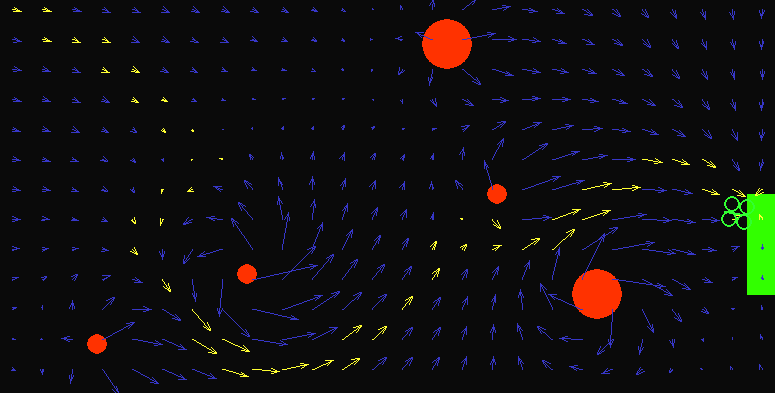
\includegraphics[width=1.0\textwidth]{img/goal_directed}
    \caption{Potential Field, leading a drone towards a goal (simple simulation)}
    \label{fig:goal_directed}
  \end{figure}


\subsection{Reinforcement Learning}
% - updating vectors
% - values
\paragraph{Exploration}
A parameter $\epsilon$ is set that determines the amount of exploration. During an exploration step, instead of the actual nearest force vector a random force vector is created and used until a next force vector is reached.

\paragraph{Value Update}
The return function $r(\vec{F})$ returns a positive value when a goal is reached, a negative value when hitting a obstacle and zero otherwise. To use the reward information for estimating the expected long-term return, each vector is extended with a \emph{(potential) value} $V$. This value is being used for the expected return value\footnote{see section \ref{sec:future} on future research for an alternative approach}, and is necessary for temporal difference used by the vector update.

The value corresponding to the last force vector $\vec{F}_{t-1}$ is updated each time a new force vector $\vec{F}_t$ is being used using TD:
 \[ V(\vec{F}_{p-1}) \leftarrow V(\vec{F}_{p-1}) + \alpha [ r(\vec{F}_p) + \gamma V(\vec{F}_p) - V(\vec{F}_{p-1}) ] \]
or
 \[ V(\vec{F}_{p-1}) \leftarrow (1 - \alpha) V(\vec{F}_{p-1}) + \alpha ( r(\vec{F}_p) + \gamma V(\vec{F}_p) ) \]
where $\vec{F}_{p-1}$ stands for the last force vector being used (with $p-1$ the previous force vector position).


\paragraph{Vector Update}
The force vector will be updated as a weighted sum of the force vector and the speed vector that was actually flown\footnote{If the inertia would become stronger on high speeds, one could calculate the force vector that would be needed to fly the speed vector and use the result, instead of the speed vector.}.
% TODO: hier over nadenken: in feite vlieg je de vector die is opgegeven, dus ff == sv (behalve bij exploration of hoge speed)

Paths that result in high returns were (obviously) better than paths that result in lower returns. Therefore speed vectors that increases the (potential) value $V$ more should be weighted more than speed vectors that increase $V$ less. Paths resulting in a negative return get a negative difference value, which effectively points the weighted speed vector to the opposite direction.

The vector update follows:
 \[ \vec{F}_{p-1} \leftarrow (1 - \lambda) \vec{F}_{p-1} + \lambda \vec{S}_{p-1} \]
where $\vec{S}_{t-1}$ stands for the previous speed vector, and $\lambda$ determined by $\alpha$ and the temporal difference:
 \[ \lambda = \alpha (V(\vec{F}_p) - V(\vec{F}_{p-1})) \]
 It is important that the values do not exceed the boundaries -1 and 1 if there is no maximum speed set, since otherwise the force vectors could increase their length to high values not only due to long speed vectors, but also due to high TD and $\lambda$ weights.
 
% TODO: nog eens goed over nadenken

A history of the last $H$ used force vectors could be remembered and used to update a couple of vectors back each time based on the temporal difference between the value of the current vector and the value of each vector $h$ steps back in history divided by the number of vectors $h$, setting lambda to:
 \[ \lambda = \alpha \frac{ V(\vec{F}_p) - V(\vec{F}_{p-h}) }{ h } \]
Using this history update faster learning could be obtained with less episodes needed for reasonable results.


\subsection{Figure-eight}

% - field description
% - static environment (but RL could solve changes, probably also extra forces when new objects are detected)
% - 2D problem, but 3D should work since all theory uses vectors
The goal of the Figure-eight task is to move in a figure-8 around two poles (figure \ref{fig:pylonchallenge}). The task occurs in a static environment and is essentially a 2D problem, although the used method should work equally well in 3D since general vectors are being used in all formulas. We will discuss some difficulties concerning the use of the framework we talked over until now, and show the steps being accomplished to define the figure-eight task into the framework.

  \begin{figure}
    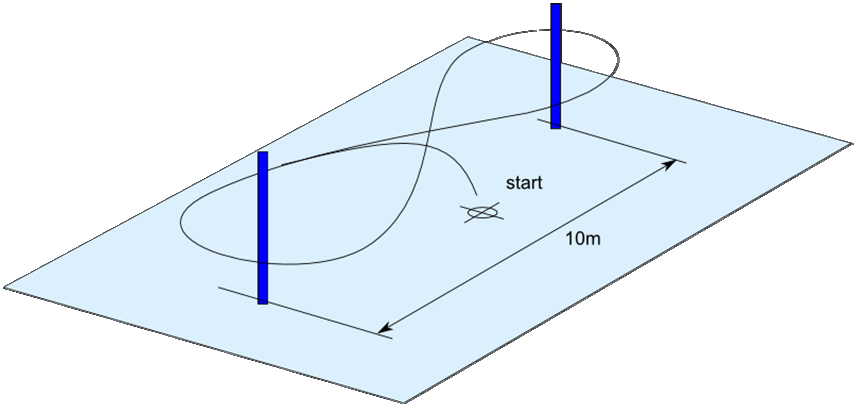
\includegraphics[width=1.0\textwidth]{img/imav2011_pylon}
    \caption{Figure-eight pylon challenge}
    \label{fig:pylonchallenge}
  \end{figure}

\paragraph{Force Fields}
% - stages
% - transitions
One difficulties in using a potential field is the continue characteristic, which makes defining a clear target location difficult. Another one is the center of the field (between the two poles), which sometimes needs to be passed in one direction and other times in the other direction. Both difficulties are solved by introducing two different \emph{stages}, one for `left to right' and one for `right to left'. Each stage has its own stage \emph{transition} which is defined as passing the line through both poles at the outside of the corresponding pole (right or left). Each stage has its own force field too, enabling the robot to learn different forces for the same locations, depending on the current location of the target line.

\paragraph{Reinforcement Learning}
% - RL
The reward function returns 1 for a state transition and -1 for a collision. The reinforcement learning occurs within stages and is restarted after a transition, as a result of which the values fall from almost 1 to possibly lower than 0 without getting problems with these large negative temporal differences. A lot of runs will then change the force fields by using the value and vector update rules.



%%%% Practical Tests %%%%
\section{Practical Tests}
\label{sec:tests}

%todo

\subsection{Simple Simulation}

\subsection{USARSim simulation}

\subsection{IMAV2011 \& AR.Drone}



% IMPLEMENTATION? if so, change end of motivation



%%%% Results %%%%
\section{Results}
\label{sec:results}

%todo
% - images

\subsection{Simple Simulation}

\subsection{USARSim Simulation}

%\subsection{Real-World}



%%%% Conclusion / Discussion %%%%
\section{Conclusion \& Discussion}
\label{sec:conclusion}
%todo

% - limitations
%   * trajectories between narrowly spaced obstacle
%   * oscillations
%   * inertia of robot (more speed = more problems; more air resistance = better)


%%%% Future Research %%%%
\section{Future Research}
\label{sec:future}
%todo

% - transition to real-world (direct location with slam+map without scale, big map without scale, relevant features such as distance to pylon (not visualizable) for which initial field could be set)
% .....
% .....
% - check mathematically (convergence, etc)
% - incorporating the vector length and value function (for constant speed)


%%%% Bibliography %%%%
%todo
\bibliographystyle{plain}
\bibliography{Thesis}




\end{document}

